\documentclass[12pt,a4paper]{article}
\usepackage{graphicx}
\usepackage[czech]{babel}
\usepackage[utf8]{inputenc}
\usepackage{titling}
\usepackage{pdfpages}
\usepackage[nopar]{lipsum}
\usepackage{mathtools}
\usepackage{multirow}
\usepackage{caption}
\usepackage{float}
\usepackage{enumitem}
\usepackage{listings}
\usepackage{amsmath}
\usepackage{amssymb}
\usepackage[left=25mm,right=25mm,top=30mm,bottom=20mm]{geometry}
\bibliographystyle{abbrv}




\begin{document}
\title{SLAM - rešerše \\ Projekt 4}
\author{Jakub Kratochvíl}
\date{Akademický rok 2017/2018}
\begin{titlepage}
\begin{center}

\includegraphics[scale=0.5]{logo_zcu}\\
\vspace{5cm}
\begin{Large}
\textbf{\thetitle}\\
\end{Large}
\vspace{3cm}
\theauthor\\
\vspace{5cm}
\thedate
\end{center}
\end{titlepage}
\newpage
		
		
\tableofcontents
\newpage
\fontsize{12pt}{18pt}\selectfont


\section{Úvod}
SLAM je zkratka pro simultánní lokalizaci a mapování, jeden ze základních problémů autonomních robotů. Jeho řešením by měl být robot, schopný na neznámém místě v neznámém prostředí vytvořit mapu tohoto prostředí a zároveň se v ní sám během pohybu lokalizovat.

Do povědomí se SLAM dostal v roce 1986 na konferenci IEEE Robotics and Automation, která se konala v San Francisku v Kalifornii \cite{Durrant-Whyte}. V tomto období se v robotice a umělé inteligenci začaly objevovat metody založené na pravděpodobnostních principech a tak vyvstala otázka možnosti použití odhadových metod na mapovací a lokalizační problémy. Po následujících diskuzích se problém ukázal jako velice zajímavý a konzistentní pravděpodobnostní mapování stalo jedním ze základních problémů a výzev robotiky.

Aplikací SLAM můžeme najít mnoho, počínaje autonomním domácím vysavačem nebo sekačkou na trávu přes robotický průzkum opuštěných nebo člověku nebezpečných prostor, navigaci ponorek kolem podmořských přírodních překážek, řízení bezpilotních letounů a dronů až po v poslední době hodně diskutované samořídící automobily nebo dokonce planetární rovery brázdící povrch Marsu.

Tato práce si klade za úkol čtenáře seznámit se základními vlastnostmi a popisem problému SLAM. Dává nahlédnout do jeho původní pravděpodobnostní definice a v další části se podrobněji zabývá metodou Graph SLAM. 


\newpage
\section{SLAM}
SLAM je problém týkající se otázky, zda je možné najít polohu nějakého zařízení vzhledem k jeho okolí a současně mapovat strukturu prostředí.

Landmarky nebo také majáky jsou nezaměnitelné a snadno rozpoznatelné orientační body v prostředí, které mohou být v některých aplikacích dopředu známy. Například autonomní vozík pohybující se ve výrobní hale může mít předem nadefinovanou mapu landmarků. Nebo robot pro práci pod širým nebem používající pro svou orientaci GNSS (globální družicový polohový systém). V takových případech, kdy lze stroj lokalizovat vzhledem ke známým bodům, nemusí být SLAM vyžadován. Ovšem v husté zástavbě, v podzemí a uvnitř budov je použití GNSS omezené nebo úplně nemožné. V neznámém prostředí zase nelze využít předem připravenou mapu a přichází nutnost použití jiného řešení, kterým bývá nejčastěji právě SLAM. Navíc v mnoha vojenských i civilních aplikacích není cílem lokalizace, ale právě robotem vytvořená mapa, kterou poté dále zpracovává lidský operátor.

Další z impulzů vývoje simultánní lokalizace a mapování byl špatný odhad pohybu získaný z odometrie kol, čímž se rozumí například počet otáček, úhel natočení apod. \cite{Past_Present_and_Future_of_Simultaneous_Localization_And_Mapping}. Tento odhad se navíc s ujetou vzdáleností zhoršuje (tzv. drift) a tím znemožňoval použití pro správnou a přesnou lokalizaci i tvorbu mapy. Nicméně dnešní algoritmy dokáží snížit drift na přijatelnou hodnotu 0,5\% a méně, takže v tomto ohledu není nutno využívat SLAM. \\ V čem je ale stále nenahraditelný, je schopnost tzv. uzavírání smyček. Při použití dat pouze z odometrie robot vnímá svět jako "nekonečný koridor", ve kterém neustále zkoumá nové oblasti (obr.1 vlevo). SLAM ale dokáže robotem vytvořenou smyčku uzavřít, protože porovná aktuální landmarky s těmi dříve objevenými a tím dokáže správně porozumět topologii prostředí a v mapě určit, že tyto dvě chodby se protínají (obr.1 vpravo).

\begin{figure}[H]
\centering
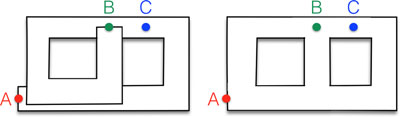
\includegraphics[scale=1]{Obr1} 
\caption{Levá mapa je vytvořená pomocí odometrie a znázorňuje jeden dlouhý koridor od bodu A do B. Body, které jsou ve skutečnosti blízko (B a C) mohou být podle této mapy libovolně daleko. Pravá mapa je vytvořená pomocí SLAM s využití uzavírání smyček, kde je znázorněná správná topologie prostředí, neboť robot správně našel "zkratku" mezi dvěma koridory. \cite{Past_Present_and_Future_of_Simultaneous_Localization_And_Mapping}}
\end{figure}


\newpage
SLAM je ze své podstaty problém typu slepice-vejce a je tedy do značné míry netriviální. Robot pro svoji lokalizaci potřebuje mapu terénu, avšak k sestavení mapy musí znát svou vlastní polohu. Ovšem existují algoritmy, které, i přes tento rozpor, uspokojivě fungují a nasnadě je tedy otázka "Je SLAM vyřešen?". Ano i ne, otázku je nutno položit pro konkrétní konfiguraci robota, prostředí a požadavků, kde může figurovat mnoho kombinací, např. z následujících možností.
\begin{itemize}
\item Robot: dynamika, maximální rychlost, dostupné senzory, výpočetní výkon
\item Prostředí: 2D/3D, přírodní/umělé, přítomnost dynamických prvků, množství a typ landmarků, množství symetrie
\item Požadavky: přesnost odhadu stavu robota, přesnost a typ mapy, míra úspěšnosti, latence odhadu, maximální velikost mapované oblasti...
\end{itemize}
Například mapování vnitřního 2D prostředí s robotem vybaveným snímačem kol a laserovým senzorem s dostatečnou přesností a robustností lze považovat z velké části za vyřešené. Na druhou stranu další kombinace robot/prostředí/požadavky si stále zaslouží velké množství výzkumu. Aktuální algoritmy mohou snadno selhat, jestliže je pohyb robota nebo prostředí příliš náročný.


\section{Pravděpodobnostní definice}
Uvažujme mobilního robota, který se pohybuje v neznámém prostředí a pomocí svých senzorů pořizuje relativní pozorování okolních landmarků (obr.2).

\begin{figure}[H]
\centering
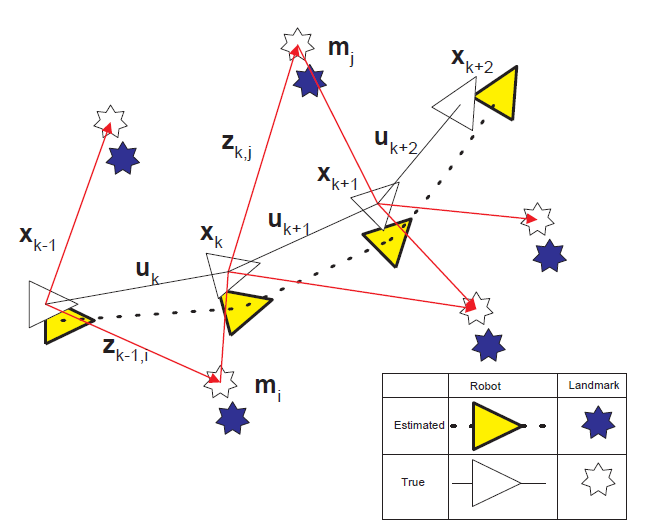
\includegraphics[scale=0.6]{Obr2}
\caption{Skutečné umístění landmarků ani robota není nikdy známo, jen jejich vzájemná poloha \cite{Durrant-Whyte}.}
\end{figure}

V okamžiku \textit{k} definujeme následující veličiny a zároveň vektory jejich historie od počátku snímání až do aktuálního časového kroku:
\begin{itemize}
\item \textbf{x}$_k$; \textbf{X}$_{0:k}=\lbrace \text{x}_0, \text{x}_1,\cdots, \text{x}_k\rbrace = \lbrace \textbf{X}_{0:k-1}, \textbf{x}_k \rbrace$:  
Stavový vektor popisující polohu a orientaci robota, respektive  historii všech jeho stavů.
\item \textbf{u}$_k$; \textbf{U}$_{0:k}=\lbrace \text{u}_1, \text{u}_2,\cdots, \text{u}_k\rbrace = \lbrace \textbf{U}_{0:k-1}, \textbf{u}_k \rbrace$: 
Vektor řízení použitý v čase \textit{k}-1 pro dosažení stavu x$_k$ v čase \textit{k}, resp. historie řízení.
\item \textbf{m}$_i$; $\textbf{m}=\lbrace \text{m}_1, \text{m}_2,\cdots, \text{m}_n\rbrace$: 
Vektor popisující polohu i-tého landmarku, resp. vektor popisující polohy všech landmarků.
\item \textbf{z}$_{ik}$; \textbf{Z}$_{0:k}=\lbrace \text{z}_1, \text{z}_2,\cdots, \text{z}_k\rbrace = \lbrace \textbf{Z}_{0:k-1}, \textbf{z}_k \rbrace$: 
Pozorování o poloze i-tého landmarku získané z robota, resp. soubor všech pozorování.
\end{itemize}

Skutečný robot bude vždy zatížen nějakou nepřesností použitých měřících zařízení a tak se přímo nabízí využití pravděpodobnosti pro formulaci úlohy SLAM. Tento přístup je jedním z nejběžnějších a také nejstarších. K vyřešení problému SLAM je potřeba určit sdruženou aposteriorní hustotu pravděpodobnosti landmarků \textbf{m} a stavů robota x$_k$ pro všechny časy $k$.

\begin{eqnarray}
p(\textbf{x}_k, \textbf{m} \,|\, \textbf{Z}_{0:k}, \textbf{U}_{0:k}, \textbf{x}_0)
\end{eqnarray}

K výpočtu je nutno znát vektor pozorování, vektor řízení a počáteční polohu robota. Výpočet hustoty se provádí pro každý časový okamžik $k$. Vhodné je použít rekurzivní algoritmus, který získá hustotu pravděpodobnosti v časovém okamžiku $k$ pomocí hustoty v okamžiku $k-1$.

\begin{eqnarray}
p(\textbf{x}_{k-1}, \textbf{m} \,|\, \textbf{Z}_{0:k-1}, \textbf{U}_{0:k-1})
\end{eqnarray}

Tento výpočet vyžaduje definování modelu pozorování a pohybového modelu.

\begin{enumerate}
\item \textbf{Model pozorování} popisuje s jakou pravděpodobností získáme pozorování z$_k$, pokud známe polohu robota i landmarků.
\begin{eqnarray}
p(\textbf{z}_k \,|\, \textbf{x}_k, \textbf{m})
\end{eqnarray}
\item \textbf{Pohybový model} popisuje s jakou pravděpodobností se robot nachází ve stavu x$_k$, pokud známe předchozí stav x$_{k-1}$ a aplikované řízení u$_k$.
\begin{eqnarray}
p(\textbf{x}_k \,|\, \textbf{x}_{k-1}, \textbf{u}_k)
\end{eqnarray}
\end{enumerate}

Stavový přechod pohybového modelu je Markovský proces, neboť stav x$_k$ závisí pouze na předchozím stavu x$_{k-1}$ a aplikovaném řízení u$_k$ a je nezávislý na pozorováních i mapě. SLAM algoritmus je nyní implementován ve standardní dvoustupňové (predikce-korekce) rekurzivní formě.

\newpage



\begin{enumerate}
\item \textbf{Predikce} 
\begin{eqnarray}
p(\textbf{x}_k, \textbf{m} \,|\, \textbf{Z}_{0:k-1}, \textbf{U}_{0:k}, \textbf{x}_0) \: = 
\end{eqnarray}
$$
= \: \int p(\textbf{x}_k \,|\, \textbf{x}_{k-1}, \textbf{u}_k) \: \times \: p(\textbf{x}_{k-1}, \textbf{m} \,|\, \textbf{Z}_{0:k-1}, \textbf{U}_{0:k-1}, \textbf{x}_0) d\textbf{x}_{k-1}  
$$
\item \textbf{Korekce}
\begin{eqnarray}
p(\textbf{x}_k, \textbf{m} \,|\, \textbf{Z}_{0:k}, \textbf{U}_{0:k}, \textbf{x}_0) \: = \: \frac{p(\textbf{z}_k \,|\, \textbf{x}_k, \textbf{m}) p(\textbf{x}_k, \textbf{m} \,|\, \textbf{Z}_{0:k-1, \textbf{U}_{0:k}, \textbf{x}_0})}{p(\textbf{z}_k \,|\, \textbf{Z}_{0:k-1}, \textbf{U}_{0:k})}
\end{eqnarray}
\end{enumerate}

Rovnice (5) a (6) poskytují rekurzivní postup pro výpočet hustoty pravděpodobnosti $p(\textbf{x}_k, \textbf{m} \,|\, \textbf{Z}_{0:k}, \textbf{U}_{0:k}, \textbf{x}_k)$ stavu robota \textbf{x}$_k$ a mapy \textbf{m} v čase $k$ na základě všech pozorování \textbf{Z}$_{0:k}$ a všech řízení \textbf{U}$_{0:k}$.

Problém budování mapy lze formulovat jako výpočet podmíněné hustoty pravdě\-podobnosti $p(\textbf{m} \,|\, \textbf{X}_{0:k}, \textbf{Z}_{0:k}, \textbf{U}_{0:k})$. To předpokládá, že umístění robota \textbf{x}$_k$ je známo (nebo alespoň deterministické) po celou dobu, pod podmínkou znalosti počátečního umístění. Mapa \textbf{m} se potom vytvoří spojením pozorování z různých míst. Naopak problém lokalizace může být formulován jako výpočet pravděpodobnostní distribuce $p(\textbf{x}_k \,|\, \textbf{Z}_{0:k}, \textbf{U}_{0:k}, \textbf{m})$. To předpokládá, že je známo umístění landmarků a cílem je vzhledem k nim vypočítat odhad umístění robota. Avšak model pozorování $p(\textbf{z}_k \,|\, \textbf{x}_k, \textbf{m})$ závisí jak na stavu robota, tak na umístění landmarků. Z toho vyplývá, že pravděpodobnostní hustota nelze takto rozdělit
$$
p(\textbf{x}_k, \textbf{m} \,|\, \textbf{z}_k) \: \ne \: p(\textbf{x}_k \,|\, \textbf{z}_k)p(\textbf{m} \,|\, \textbf{z}_k).
$$
Takové rozdělení by vedlo k nekonzistentnosti odhadů a nepoužitelným výsledkům. 

\section{Graph-Based SLAM}
Při tomto přístupu se k ukládání dat používá graf. Uzel grafu reprezentuje stav robota a měření provedená z tohoto stavu. Hrany mezi uzly představují jejich vzájemnou polohu. Cílem algoritmu je najít takové rozložení uzlů, které minimalizuje čtvercovou chybu rozdílu pozorování a "virtuálního pozorování" \cite{GraphSLAM}. Tím se získá nejlepší odhad mapy. Optimalizace neprobíhá po každém novém pozorování, čímž se Graph SLAM řadí mezi offline metody řešení.

Formulace SLAM pomocí grafu byla poprvé představena v roce 1997, avšak kvůli vysoké výpočetní náročnosti trvalo ještě několik let, než se začala používat v reálných aplikacích. V dnešní době patří Graph SLAM k nejmodernějším technikám, co se rychlosti a přesnosti týče.

\subsection{Definice}
Pro správný chod graph SLAMu musí fungovat souhra mezi jeho dvěma částmi front-end a back-end. Front-end se obecně stará o sestrojení samotného grafu a back-end o jeho optimalizaci a tedy i optimalizaci mapy.

\begin{figure}[H]
\centering
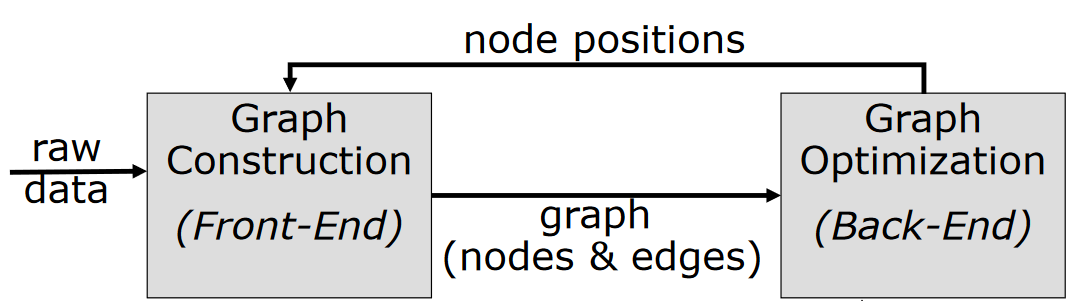
\includegraphics[scale=0.5]{Obr3}
\caption{Schéma převzaté z \cite{16-graph-slam} znázorňuje průchod dat metodou Graph SLAM. Surová data (pozorování, odometrie) nejdříve zpracuje front-end a vytvoří graf. Ten po daném okamžiku putuje do back-end, kde se optimalizací získá nejlepší odhad mapy prostředí a poté předá opět do první části.}
\end{figure}

\subsubsection{Front-end}
První část vytváří graf, kterým reprezentuje mapu prostředí. Každý uzel $x_i$ obsahuje informaci o stavu robota a o pozorování provedeném z tohoto stavu v čase $i$. Hrana mezi sousedními uzly $x_i$ a $x_{i+1}$ odpovídá zaznamenané odometrii při pohybu robota. Pokud je hrana mezi různými uzly $x_i$ a $x_j$, pak je to tzv. virtuální měření. To se zaznamená ve chvíli, kdy robot naměří podobná data (tzn. ocitne se ve stejné části prostředí) jako v některém z předešlých měření. 

Využívá se scan matching, který porovnává dvě pozorování z uzlů $x_i$ a $x_j$ z různých časových okamžiků a v případě zjištění podobnosti je vypočítána relativní poloha uzlů $x_i$ a $x_j$. To je ve skutečnosti transformace pozorování z $x_i$ taková, aby se maximálně překrývalo s pozorováním uzlu $x_j$. Tuto transformaci nazýváme virtuálním pozorováním.

Znázornění problému je v obrázku 4, kde $x_i$ je aktuální uzel, $x_j$ je uzel, ve kterém bylo provedeno podobné pozorování jako to aktuální, $\hat{z}_{ij}$ je predikce virtuálního měření reprezentující "jak uzel $i$ vidí uzel $j$", $z_{ij}$ je virtuální měření, $\Omega_{ij}$ je informační matice virtuálního měření a $e_{ij}(x_i, x_j)$ je funkce, která vyjadřuje rozdíl virtuálního a predikovaného měření.
\begin{figure}[H]
\centering
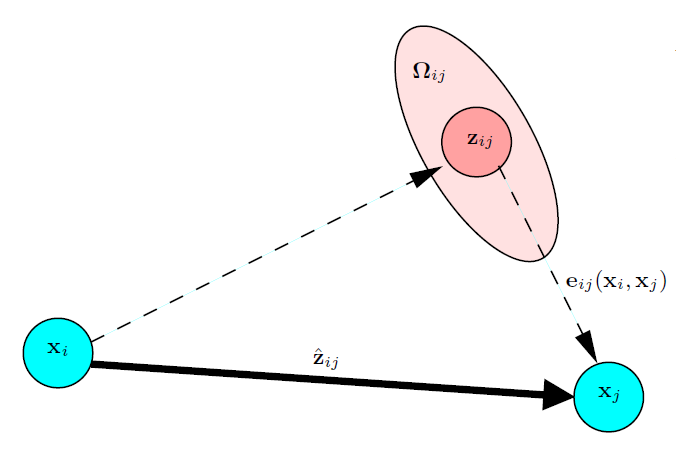
\includegraphics[scale=0.8]{Obr4}
\caption{Znázornění virtuálního měření a jeho predikce \cite{tutorialGraph}.}
\end{figure}



\subsubsection{Back-end}
Druhá část se stará o optimalizaci rozložení uzlů v grafu.

Definujme funkci 
$$
\textbf{e}_{ij}(\textbf{x}_i, \textbf{x}_j) \: = \: \textbf{z}_{ij}-\hat{\textbf{z}}_{ij}(\textbf{x}_i, \textbf{x}_j),
$$
která vyjadřuje chybu mezi predikcí měření $\hat{\textbf{z}}_{ij}$ a měřením $\textbf{z}_{ij}$ a je také znázorněna v obrázku 4. Optimalizace rozložení všech uzlů dosáhneme minimalizací funkce $\textbf{F}(\textbf{x})$ pro všechna virtuální měření
$$
\textbf{F}(\textbf{x}) \: = \: \sum\limits_{i,j} \textbf{F}_{ij} \: = \: \sum\limits_{i,j} \textbf{e}_{ij}^T \Omega_{ij} \textbf{e}_{ij}.
$$
Nejlepší odhad mapy tedy musí splňovat podmínku
$$
\textbf{x}^* \: = \: \text{argmin}\, \textbf{F}(\textbf{x}).
$$
Numericky lze tento problém řešit metodou nejmenších čtverců, konkrétně na odhad rozmístění uzlů z front-end aplikovat Gauss-Newtonův algoritmus, který minimalizuje chybovou funkci $\textbf{e}_{ij}(\textbf{x}_i, \textbf{x}_j)$.


\section{Vizuální SLAM}
Vizuální SLAM, Visual-based SLAM nebo také vSLAM je přístup k simultánní lokalizaci a mapování, při kterém jsou jako vstup algoritmu využívány obrazová data. Tato metoda se začala používat až po roce 2000, neboť zpracování obrazu z kamery je značně výpočetně náročné. 

Na druhou stranu sebou přináší dodatečné informace o vzhledu, barvě, jasu a textuře prostředí. To umožňuje začlenění dalších úkolů jako například detekce a rozpoznávání obličeje, věcí nebo konkrétních míst. Pro vSLAM také nahrává cenová dostupnost kamer, jejich velikost a nižší spotřeba energie oproti často používaným laserovým skenerům. 

Bohužel při použití snímačů obrazových dat mohou vzniknout chyby pokud kamera nemá dostatečné rozlišení, v prostředí je málo nebo moc landmarků, snímané povrchy nemají nedostatečnou texturu, málo osvětlení a jeho změny nebo pořízení rozmazaných snímků při pohybu. Navíc nezávisle na použitém algoritmu musí být provedena kalibrace kamer.

\subsection{Základní struktura vSLAM}
Většina vSLAM algoritmů používá stejnou obecnou strukturu, která se skládá ze tří hlavních částí:
\begin{itemize}
\item Kalibrace  
\item Sledování
\item Mapování
\end{itemize}

Nezávisle na přesném typu algoritmu musí proběhnout kalibrace kamer. Ta se dá rozdělit na vnitřní, která odpovídá geometrii kamery (ohnisková vzdálenost) a vnější, která záleží na pozici kamery v prostoru (rotace a translace s respektováním nějakého souřadnicového systému). Provádí se s použitím několika různých obrazů s motivem šachovnice. Jejich nasnímáním se vnitřní souřadnicový systém nastaví tak, aby odpovídal reálnému světu.

V další části je sledovaný obraz zasazen do rekonstruované mapy k odhadu pozice robota. K tomu je potřeba nejdříve najít společné významné body obrazu s mapou a poté vypočítat odhad pozice kamery.

Mapováním se rozumí rozšiřování existující mapy v případě, kdy kamera zachytí dosud neznámou oblast.

\subsection{Dodatkové moduly vSLAM}
Následující dvě části jsou často zahrnuty do algoritmu pro stabilnější a přesnější běh, avšak v závislosti na konkrétním použití je lze vynechat:
\begin{itemize}
\item Relokalizace
\item Globální optimalizace mapy
\end{itemize}

V případě, kdy robot ztratí přehled o své pozici, například kvůli rychlému pohybu kamery, je zapotřebí jej znovu lokalizovat. Pokud by vSLAM systém neobsahoval tuto funkci, nemohl by dále pokračovat po ztrátě informace o své pozici.

Mapa zpravidla obsahuje kumulativní chybu odhadu, která se zvětšuje s ujetou \linebreak vzdáleností. Když robot navštíví již dříve objevenou oblast, použitím techniky zvané uzavírání smyček, dojde k porovnání aktuálního obrazu s dříve nasnímanými a v případě shody může být dopočítána a následně odstraněna chyba odhadu.

\subsection{Metody řešení}
Existují tři základní přístupy v získávání a/nebo zpracování obrazových dat. První dva rozlišujeme podle práce s obrazovými daty, kdy jeden přístup je založen na detekci a zpracování významných bodů, zatímco druhý pracuje přímo se získaným obrazem. Třetí možností je použití RGB-D kamer jako je například Microsoft Kinect, který je výhodný v možnosti získávání nejen obrazu prostředí, ale i informaci o jeho hloubce. 

\subsubsection{S použitím významných bodů}
První monokulární SLAM nazvaný MonoSLAM byl vyvinutý v roce 2003. V tomto algoritmu probíhá lokalizace i mapování souběžně a k odhadu se používá Kalmanův filtr. Pohyb kamery a pozice významných bodů prostředí jsou reprezentovány stavovým vektorem. Při objevení nového významného bodu je tento přidán do stavového vektoru, v důsledku čehož se při použití ve velkém prostředí dimenze vektoru zvětší natolik, že výpočetní náročnost souběžné lokalizace a mapování přestává být únosná a je těžké dosáhnout potřebných odhadů v reálném čase.

Řešením problému výpočetní náročnosti je lokalizaci a mapování spustit každé na svém vlastním procesorovém vlákně tak, jako v metodě zvané PTAM (tj. Parallel Tracking and Mapping). Tyto vlákna běží paralelně, tím nedochází k omezování lokalizace výpočetní náročností odhadu mapy. Navíc je do mapování zahrnuta i průběžná optimalizace, takže je robot v reálném čase lokalizován a navíc vytvářena přesná mapa prostředí. PTAM je první metodou, která zahrnuje optimalizaci do algoritmu v reálném čase a většina novějších algoritmů následuje tento vícevláknový přístup \cite{Taketomi_visual}.

PTAM, narozdíl od MonoSLAM, dokáže v réálném čase fungovat i v případě rozlehlého prostředí, kde stavový vektor obsahuje několik tisíc významných bodů.

\subsubsection{RGB-D}
RGB-D SLAM se začal nejvíce používat po příchodu kamery Microsoft Kinect, která započala malou \uv{revoluci} díky své ceně, velikosti a jednoduchosti použití. Má zabudovanou RGB i infrakameru a dokáže tak kromě obrazu navíc získávat informaci o hloubce prostředí. Většina spotřebitelských RGB-D kamer je však určena pouze pro použití v interiéru, neboť v exteriéru je obtížné zachytit odražené IR záření a kromě toho mají malý dosah v řádu jednotek metrů.

Pomocí RGB-D kamer lze získat přímo 3D strukturu prostředí, většina přístupů však mapu rekonstruuje z kombinací více hloubkových map. K odhadu pozice kamery je hojně využívaný iterativní algoritmus nejbližšího bodu (ICP). 

\subsubsection{Přímé metody}
Přímé metody zpracovávají vstupní obraz bez použití doplňků extrahujících určité části obrazu a používají tak jeho fotometrickou konzistenci. Metody s detekcí významných bodů využívají geometrické konzistence obrazu.

Jedním příkladem je metoda DTAM, kde při lokalizaci porovnáváme vstupní obraz s uměle generovaným obrazem z rekonstruované 3D mapy. Tento algoritmus bývá implementován na grafické kartě, čímž dosáhneme vyšší efektivity výpočtu a zároveň oddělení lokalizace a mapování. Mapování se provádí s využitím několika sérií pozorování z různých míst a následnou optimalizací. Tímto způsobem lze získat všechny 3 souřadnice každého pixelu a sestavit tak 3D mapu prostředí. DTAM je navržený pro rychlé a online 3D modelování pro použití s mobilním telefonem.

LSD-SLAM











\bibliography{zdroje}




\end{document}